\documentclass{paper}
\usepackage{graphicx}
\usepackage{url}
\usepackage[utf8]{inputenc}

\title{Research-Notes}
\author{Sameer Al Harbi}

\begin{document}
\part{WolfRam 3D Plots}
\today
\begin{quote}
\url{https://reference.wolfram.com/language/howto/PlotDataIn3D.html}
\end{quote}
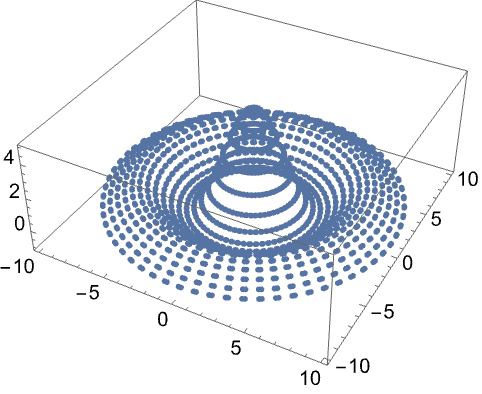
\includegraphics[width=180pt]{plot1.png}
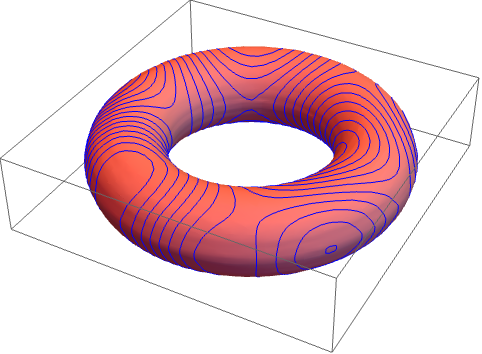
\includegraphics[width=180pt]{plot2.png}
\\
\\
\emp{WolfRam is a language and set of tools used for the computation of data. One feature of the language itself though is it's integrated ability to display 3D plots of data out of array like data points. Further effects can also be applied to create other visuals 

data1 = Flatten[
   Table[{r Cos[t], r Sin[t], 5 Sinc[r]}, {r, 0, 10, 0.5}, {t, -Pi, 
     3 Pi, 0.1}], 1];
data2 = ExampleData[{"Geometry3D", "Torus"}, "VertexData"];
}
\\
\\
\textbf{Key Points to takeaway from this}
\begin{enumerate}
    \item Consider how data is defined for wolfram to create 3D plots and consider a similar input structure
    \item consider a system to take these raw inputs and define them so WebGL or other low level API can render it
    
\end{enumerate}







\end{document}
